%%This is a very basic article template.
%%There is just one section and two subsections.
\documentclass{article}

\usepackage{amsmath}
\usepackage{amsfonts}
\usepackage{parskip}
\usepackage{cleveref}
\usepackage{xcolor} 
\usepackage{graphicx}
\usepackage{tikz}
\usepackage{pgfplots}

\setlength{\parskip}{0.2cm}

\title{TTIC 31230 Project Report}

\author{Hao Jiang}
\begin{document}

\maketitle

\section*{Introduction}
I am interested in RNN architecture related questions and would 
like to address this kind of problem in the project. More specifically,
I want to understand how multi-layer RNNs can improve the performance
comparing to single-layer RNN and how the different ways of connecting
layers would make a difference.

A typical RNN structure is demonstrated in \Cref{fig:lstm}. It comprised 
of multiple LSTM (Long short-memory) cells. All the cells have the same 
structure and share the same parameter sets. The $i$-th cell takes input 
$X_i$ from external source, it also carries two internal states, namely 
the carry state $c_i$, denoted by the top horizontal line, and hidden state
$h_i$, denoted by the bottom horizontal line. The cell makes computations 
based on the input and states, then emits the updated states $c_{i+1}$ and 
$h_{i+1}$ to next cell. The output of each cell is computed based on the 
hidden state $h_{i+1}$. 

\begin{figure}
\centering
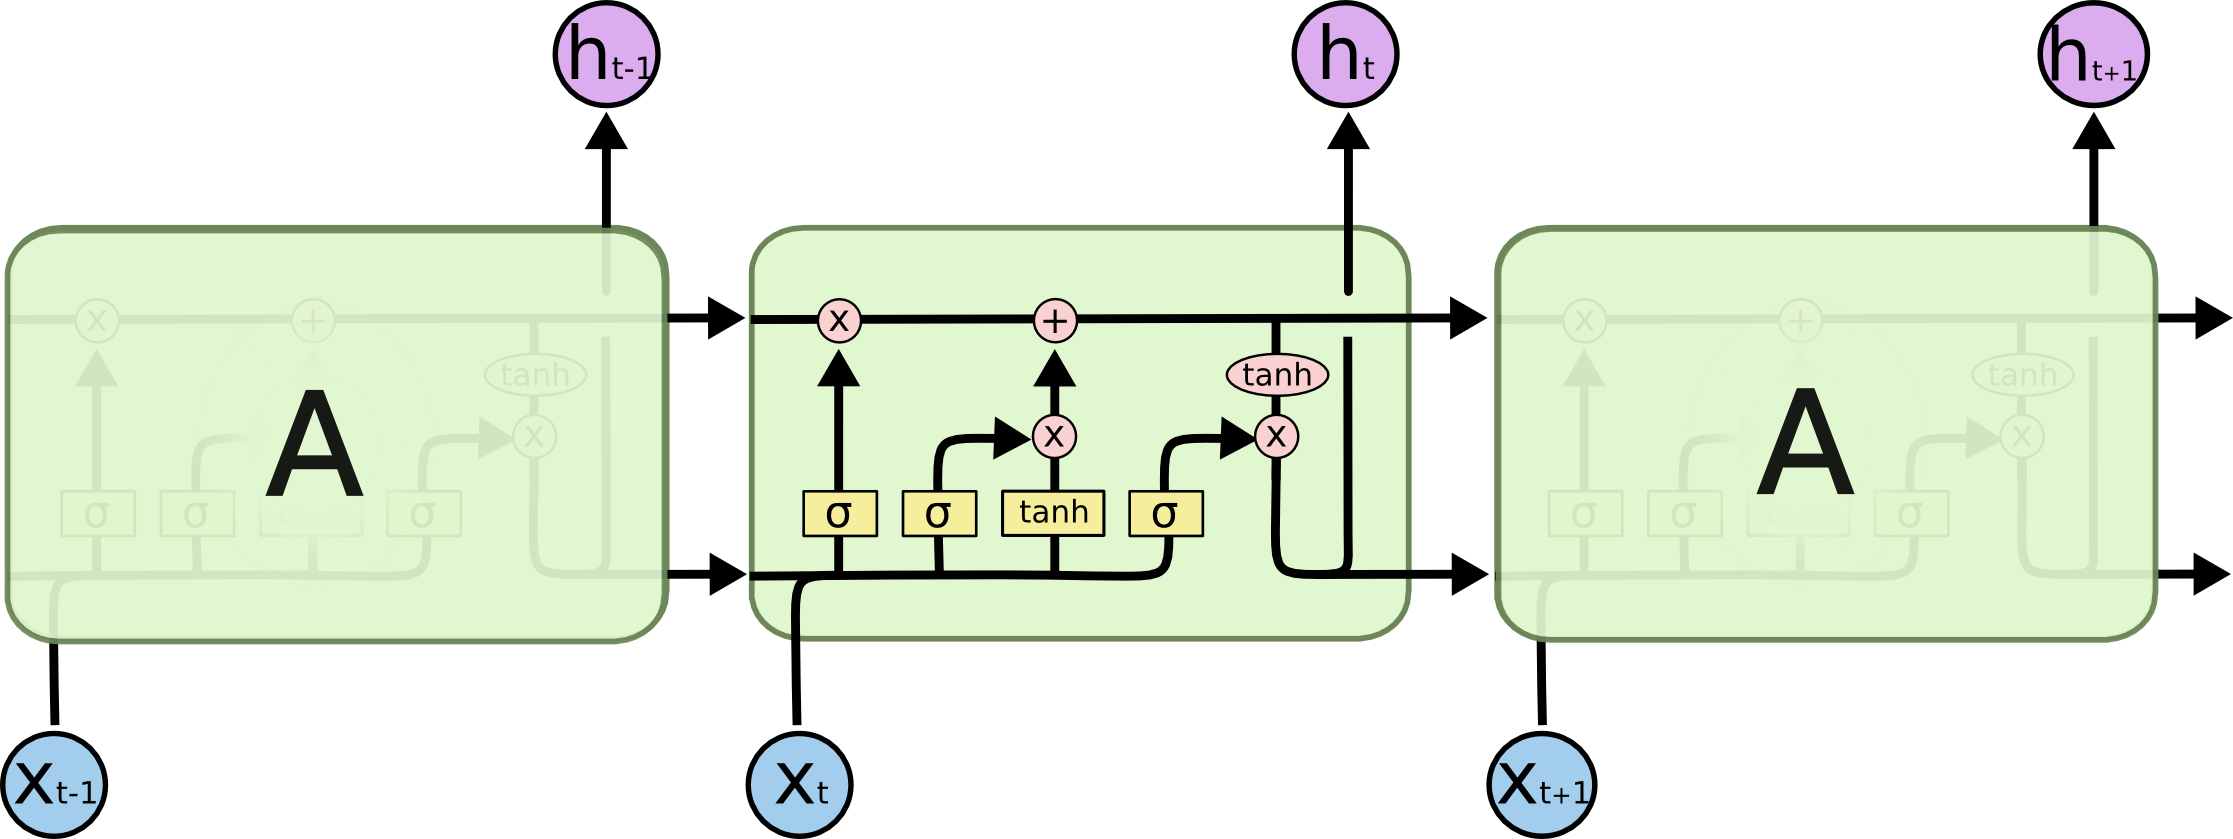
\includegraphics[scale=0.35]{lstm.png}
\caption{RNN Structure (Source: http://colah.github.io/posts/2015-08-Understanding-LSTMs/)}
\label{fig:lstm}
\end{figure} 

RNN has gained significant improvement in sequence data processing mostly
due to its special architecture. The carry state connecting LSTM cells serves
as the memory of RNN. In each step, the memory can be forgotten, or enhanced
based on both the new input and the hidden state. The output of each cell also
depends on the carry state of current cell.

A natural extension of RNN is the multi-layer RNN. A single layer RNN only
extends the network in 1-d dimension, while multi-layer RNN allows the network
to expand on 2-d dimensions. The upper layer RNN maintains its own carry state, 
and will take the hidden state from the layer below it as input. Intuitively,
this structure allows the upper layer to get summarized information from the 
lower layer and generate a more general memory state. The more layer is added
to the structure, the more general information can be captured by the top layer
of RNN.

\section*{Experiment}

Theoretically, adding more layers can be beneficiary to reducing the loss. However,
more layers almost certainly cost more time to train. Is the reduced loss worthy
for the extra training time? In additional, increasing the hidden dimension size
should also reduce loss at the cost of training time. Which method is more efficient?

To answer these questions, I conducted a series of experiments that varies both
the number of layers and the size of hidden dimensions. The experiment
parameters are listed in \Cref{tab:param}. The table shows how many epoches are 
executed for each layer and hidden dimension combination.

\renewcommand{\arraystretch}{1.2}
\begin{table}
\centering
\begin{tabular}{c|c|c|c|c}
\textbf{Layer\textbackslash HD} & 200 & 300 & 400 & 600\\
\hline
2 & 90& 90& 90& 30 \\
\hline
3 & 90& 90& 90& 30 \\
\hline
4 & 90& 90& 90& - \\
\end{tabular}
\caption{Experiment Parameter}
\label{tab:param}
\end{table}

All experiments are conducted on Dell PowerEdge R630 equipped with 2 Intel Xeon
CPU E5-2670 v3 @ 2.30GHz, 128GB memory running Ubuntu 16.04. The software 
environment is Numpy 1.11.2 running on Python 3.5.2 with the latest Intel MKL
library. In this experiment I use 7 machines with a total training time of 
over 400 hours.

\begin{figure}
\centering
\begin{tikzpicture}
\begin{axis}
\addplot table[x=ep,y=l2] {data/hd_200_time};
\addplot table[x=ep,y=l3] {data/hd_200_time};
\addplot table[x=ep,y=l4] {data/hd_200_time};
\addplot table[x=ep,y=l2] {data/hd_300_time};
\addplot table[x=ep,y=l3] {data/hd_300_time};
\addplot table[x=ep,y=l4] {data/hd_300_time};
\addplot table[x=ep,y=l2] {data/hd_400_time};
\addplot table[x=ep,y=l3] {data/hd_400_time};
\addplot table[x=ep,y=l4] {data/hd_400_time};
\end{axis}
\end{tikzpicture}
\end{figure}

\begin{table}
\centering
\begin{tabular}{c|c|c|c|c}
\textbf{Layer\textbackslash HD} & 200 & 300 & 400 & 600\\
\hline
2 & 16.250& 25.223& 36.142& - \\
\hline
3 & 24.108& 38.072& 54.319& - \\
\hline
4 & 32.186& 51.019& 72.489& - \\
\end{tabular}
\caption{Average Running Time}
\label{tab:time}
\end{table}

First, we would like to explore how much more layers can actually help improving
the accuracy. 



\begin{figure}
\centering
\begin{tikzpicture}
\begin{axis}
\addplot table[x=ep,y=l2] {data/hd_200_loss};
\addplot table[x=ep,y=l3] {data/hd_200_loss};
\addplot table[x=ep,y=l4] {data/hd_200_loss};
\end{axis}
\end{tikzpicture}
\end{figure}

\begin{figure}
\centering
\begin{tikzpicture}
\begin{axis}
\addplot table[x=ep,y=l2] {data/hd_300_loss};
\addplot table[x=ep,y=l3] {data/hd_300_loss};
\addplot table[x=ep,y=l4] {data/hd_300_loss};
\end{axis}
\end{tikzpicture}
\end{figure}

\begin{figure}
\centering
\begin{tikzpicture}
\begin{axis}
\addplot table[x=ep,y=l2] {data/hd_400_loss};
\addplot table[x=ep,y=l3] {data/hd_400_loss};
\addplot table[x=ep,y=l4] {data/hd_400_loss};
\end{axis}
\end{tikzpicture}
\end{figure}

\begin{figure}
\centering
\begin{tikzpicture}
\begin{axis}
\addplot table[x=ep,y=l2] {data/hd_200_loss};
\addplot table[x=ep,y=l2] {data/hd_300_loss};
\addplot table[x=ep,y=l2] {data/hd_400_loss};
\end{axis}
\end{tikzpicture}
\end{figure}

\begin{figure}
\centering
\begin{tikzpicture}
\begin{axis}
\addplot table[x=ep,y=l3] {data/hd_200_loss};
\addplot table[x=ep,y=l3] {data/hd_300_loss};
\addplot table[x=ep,y=l3] {data/hd_400_loss};
\end{axis}
\end{tikzpicture}
\end{figure}

\begin{figure}
\centering
\begin{tikzpicture}
\begin{axis}
\addplot[color=red,mark=None] table[x=ep,y=l4] {data/hd_200_loss};
\addplot[color=blue,mark=None] table[x=ep,y=l4] {data/hd_300_loss};
\addplot[color=black,mark=None] table[x=ep,y=l4] {data/hd_400_loss};
\end{axis}
\end{tikzpicture}
\end{figure}

\begin{figure}
\centering
\begin{tikzpicture}
\begin{axis}
\addplot table[x=ep,y=l2] {data/hd_200_perp};
\addplot table[x=ep,y=l3] {data/hd_200_perp}; 
\addplot table[x=ep,y=l4] {data/hd_200_perp};
\end{axis}
\end{tikzpicture}
\end{figure}


\end{document}

